\documentclass[11pt]{article}
\usepackage{graphicx}
\usepackage{svg}
\usepackage{minted}
\usepackage{url}
\usepackage{float}
\usepackage[letterpaper, total={7in, 9in}]{geometry}

\begin{document}

\begin{titlepage}
\centering {\includesvg[width=0.3\textwidth]{logo}\par}
\vspace{1cm}
{\LARGE Universidad Nacional Autónoma de México \par}
\vspace{0.5cm}
{\Large Facultad de Ciencias \par}
\vspace{2cm}
{\Large Proyecto 1 - Modelado y Programación \par}
\vspace{0.5cm}
{\Huge Servidor y Cliente de un Chat. \par}
\vspace{2cm}
{\Large Autor: \par}
{\Large Martínez García Emilio \par}
\end{titlepage}

\noindent En este proyecto se llevó a cabo el desarrollo de una aplicación de mensajería que permitiera a varios usuarios comunicarse entre sí de forma simultánea. Empezaré entonces con la justificación de las decisiones que tomé para realizar el diseño para después explorar este último y concluir qué cambios me hubiera gustado realizar si hubiese tenido más tiempo.

\section{Introducción}
Para la implementación de este proyecto se nos proveyeron diversas restricciones con las que debía cumplir nuestro programa, entre estas se encontraban:
\begin{enumerate}
    \item El uso de \textbf{Ruby} y \textbf{Python} estaba prohibido y el de \textbf{Java} conllevaba una penalización.
    \item Uso de \textbf{Docker} para la ejecución de nuestro programa.
    \item Uso de un sistema de construcción para que \textbf{Docker} compile y ejecute el programa.
    \item Un protocolo para la comunicación entre el servidor y los clientes. 
    \item Pruebas unitarias para este protocolo. 
    \item Uso de integración continua en nuestro repositorio.
    \item El uso de la licencia \textbf{GPL3}.
    \item Un \textbf{README} con los comandos necesarios para Docker y el sistema de construcción. 
    \item Una wiki en el repositorio con la documentación generada por el sistema de construcción.
\end{enumerate}

\section{Diseño general}
En relación con el primer punto, el proceso que me llevó a elegir Rust fue el siguiente: al principio me planteé utilizar un lenguaje orientado a objetos. pero, al buscar qué opciones habían, solo pude reconocer cuatro de estos, lo que desde mi punto de vista significaba que únicamente estos eran lo suficientemente exitosos y, por tanto, agradables de utilizar, como para que yo hubiera escuchado hablar de ellos con el poco interés que le suelo plantear a lo que probablemente me dedique el resto de mi vida, sin embargo, se dió el caso de que dos de estos (\textbf{Java} y \textbf{Ruby}) implicarían una penalización en mi proyecto, lo que dejó dos opciones sobre la mesa, \textbf{C\texttt{++}} ó \textbf{C\texttt{\#}}. A pesar de que en un principio estos dos parecían ser la decisión correcta, terminé negándome a utilizar \textbf{C\texttt{++}} después de ver su sintaxis y que se recomendaba hacer dos archivos diferentes para cada parte de mi código y no me decidí por \textbf{C\texttt{\#}} porque para ese punto en el tiempo no me había enterado que el profesor decidió penalizar únicamente Java y no a todos los lenguajes interpretados en general.\\
Lo siguiente fue entonces revisar qué opciones de lenguajes estructurados existían, en este caso, las posibilidades que más me llamaron la atención fueron: \textbf{Rust}, \textbf{C} y \textbf{Go}. En realidad, no tardé mucho desde este punto en escoger \textbf{Rust} pues mis compañeros parecían inclinarse hacia este, así que me pareció buena idea utilizar un lenguaje que me permitiría obtener ayuda más fácilmente en caso de necesitarla, aunado a esto, su sistema de construcción y manejador de paquetes, \textbf{Cargo}, se veía extremadamente sencillo de utilizar y, mientras investigaba un poco más sobre el lenguaje, me enteré de que ha sido votado como el lenguaje favorito de todos los niños por muchos años consecutivos.\\\\
Una vez elegido el lenguaje que utilizaría, lo primero que hice fue crear crear tres paquetes diferentes, dos binarios que serían uno para el servidor y el otro para el cliente, y una biblioteca que tendría código relacionado al protocolo para así poder utilizarlo desde cualquiera de los dos binarios.\\
Ya que tenía un esqueleto muy sencillo de lo que iba a ser mi proyecto, lo siguiente que hice fue agregar la licencia y la integración continua a mi repositorio, afortunadamente, GitHub básicamente creó ambas automáticamente, por lo que no fue necesario poner demasiado empeño en esto.\\

\section{Diseño del protocolo}

Tomando en cuenta que tanto el servidor como el cliente dependían ampliamente del protocolo para comunicarse entre sí, decidí comenzar con la biblioteca compartida que, además, debería ser bastante sencilla de realizar.\\
La biblioteca que usé para manejar de forma más sencilla los \textbf{JSON} fue \textbf{serde} y, aunque como se puede intuir por su nombre permite serializar y deserializar estructuras y enumeraciones, estas últimas más que nada por su capacidad de tener variantes que son estructuras, me pareció que crear una estructura, serializarla, convertirla a bytes y luego mandarla iba a terminar haciendo mi código innecesariamente largo en muchas ocasiones, así que en lugar de crear estructuras serializables, decidí crear funciones que me devolvieran el \textbf{JSON} ya en un \textbf{String}. Para esto utilicé un macro que, por suerte, formaba parte de la misma biblioteca, y así logré que cada vez que quisiera mandar un mensaje mi código en lugar de verse como:

\begin{minted}{rust}
// ...
let nuevo_estado = NewStatus{ username: "Kimberly".to_string(),
                              status: Active };
let json = match serde_json::to_string(&nuevo_estado) {
    Err(_) => {},// No puede pasar
    Ok(s) => s,
};
if let Err(e) = conexion.cliente_out(json).await {
    bitacora::error(e);
    return;
}
// ...
\end{minted}
Se viera de esta forma:

\begin{minted}{rust}
// ...
if let Err(e) = conexion.cliente_out(new_status(&"Kimberly".to_string(), &Active)) {
    bitacora::error(e);
    return;
}
// ...
\end{minted}
Por otro lado, para la deserialización sí era importante poder guardar toda la información en las variantes de una enumeración personalizada por dos principales razones: primero, por omisión, serde deserializa las cadenas a una enumeración definida de la siguiente manera:
\begin{minted}{rust}
pub enum Value {
    Null,
    Bool(bool),
    Number(Number),
    String(String),
    Array(Vec<Value>),
    Object(Map<String, Value>),
}
\end{minted}
A partir de esta enumeración, sería muy complicado no solo obtener la información de cada mensaje recibido, sino también el hecho de tan siquiera asegurarnos de que fuera un mensaje válido del protocolo pues tendríamos que revisar que fuera la variante Object, que el diccionario dentro de la variante Object tuviera una entrada "type", que esta fuera un tipo válido del protocolo, que el diccionario tuviera exactamente la cantidad de entradas que el tipo asociado debe tener, que estas entradas tuvieran el mismo nombre que en el mensaje del protocolo y que las variantes de Value en cada entrada fueran válidas acorde a lo que la entrada debería contener.\\
La segunda razón fue que hacer una enumeración personalizada en que todas, o al menos la gran mayoría, de variantes fueran estructuras, permite hacer funciones que aprovechen las capacidades de deserialización de serde y, en lugar de probar a deserializar con varias estructuras hasta que una de ellas no regrese un error, podemos pedir que devuelva una instancia de la enumeración y se deserializará sin problema en la correcta si es que esta existe y arrojará un error en caso de que no. Esto es extremadamente útil porque sabemos entonces que el error solamente ocurre cuando el mensaje recibido es inválido.\\\\
Ya teniendo la forma de serializar y deserializar los mensajes enviados y recibidos, solo faltan por mencionar un par de detalles más del paquete del protocolo.
\begin{itemize}
    \item Enumeraciones complementarias:\\
    El hecho de que para los mensajes del tipo \textbf{Response} tuvieran una cantidad conocida de valores posibles para sus campos \textbf{operation} y \textbf{result}, impulsó mi decisión de hacer enumeraciones para estos dos, de esta manera reduciendo la posibilidad de que se escapara un mensaje inválido en estas sin necesidad de tener que crear una variante distinta para cada operación diferente.\\
    De forma análoga, como solamente existen tres estados válidos, fue evidente que tenía que usar una enumeración para asegurarme de que solamente se aceptaran estos al deserializar los mensajes a las variantes \textbf{Status}, \textbf{NewStatus}, \textbf{UserList} y \textbf{RoomUserList}.
    \item Función para obtener la dirección del servidor:\\
    Debido a que era necesario tanto poder cambiar el puerto y la dirección a la que se conectarían tanto el cliente como el servidor, me pareció adecuado tener una función que se dedicara a obtener estos de los argumentos del programa en la biblioteca compartida, además, de esta manera me pude asegurar que si no recibían argumentos, la dirección y el puerto por omisión de ambos serían exactamente los mismos.
\end{itemize}

\section{Diseño del Servidor}
Siendo que el servidor tiene que manejar información proveniente de varios hilos a la vez que decide a cuáles de ellos enviarles qué información proveniente de otros, el siguiente paso para mí era evidentemente hacer el servidor.\\
Mientras investigaba cómo podía hacer un servidor en \textbf{Rust}, descubrí que además de la biblioteca estándar, este cuenta con una biblioteca para manejo de hilos y sockets llamada \textbf{Tokio}, la importancia de esta vino en principio ya que en la mayoría de lugares que revisé, solían recomendarla para el manejo de una gran cantidad de hilos y, aunque supuse que en una situación realista no se deberían conectar demasiados clientes a la vez a mi servidor, me pareció buena idea utilizarla por si de casualidad a alguien se le ocurría hacerle un test de estrés (lo que en realidad sí terminó sucediendo).\\
Otro punto importante del diseño del servidor como tal son los tres diccionarios constantes que sirven para guardar los estados de los usuarios, los canales internos de los usuarios y los cuartos que existan. Los tres están declarados como una \textbf{std::sync::LazyLock} que envuelve una \textbf{tokio::sync::RwLock} que a su vez envuelve un \textbf{HashMap}, en los tres casos las llaves son cadenas, sin embargo, en el primer diccionario los valores son instancias de \textbf{EstadoUsuario}, en el segundo los valores son instancias de \textbf{tokio::sync::mpsc::Sender} (La parte del canal interno de los clientes que se dedicará a mandar mensajes al receptor) y en el tercero los valores serán instancias de \textbf{Cuarto}.
\begin{enumerate}
    \item \textbf{LazyLock}\\
    Traducida al español más o menos como cerradura floja, se llama así porque, para permitirnos tener una constante mutable en tiempo de ejecución, espera hasta ser utilizada por primera vez para ejecutar la lambda que inicializa el valor interno, asegurándose así que el compilador conoce su valor en tiempo de compilación, pero al ejecutar la lambda en tiempo de ejecución es capaz de guardar una referencia a la estructura creada y, por tanto, modificarla en tiempo de ejecución.
    \item \textbf{RwLock}\\
    Llamada así por Read-Write Lock o cerradura de lectura-escritura en español, se usa para permitir que el valor contenido en su interior sea protegido de que más de un hilo lo modifique a la vez, pero a su vez permitiendo que varios lo lean al mismo tiempo.\\
    Elegí esto en lugar de un \textbf{Mutex} (que solo permite un hilo a la vez sin importar que solamente lo quiera leer o también modificar) por la misma razón que utilicé \textbf{Tokio}, para que el servidor sea ligeramente más óptimo.
\end{enumerate}
Habiendo establecido la razón por la que utilicé esa biblioteca en lugar de la estándar y el por qué de la forma en que se declaran los diccionarios, podemos continuar con una explicación más detallada de cada una de las partes del servidor.

\subsection{Bitácora}
Aunque obviamente no es necesaria para el funcionamiento del servidor (ni viceversa, en realidad), la bitácora me fue extramadamente útil para corregir errores cuando ocurría algún problema con el servidor, pues me permitía conocer en qué momento su ejecución se vió interrumpida o qué tipo de mensajes provocaron un error en su ejecución.\\
Esta se basa en únicamente 4 componentes: 
\begin{enumerate}
    \item Mensaje de recepción
    \item Mensaje de envío
    \item Errores del servidor:\\
    Exceptuando por el error de creación del servidor, que obviamente tiene como consecuencia que se termine el programa, cualquier error que ocurre mientras el servidor se está encargando de un cliente siempre termina por hacer que lo desconecte, entonces importa más que estos estén bien definidos en la bitácora, pues esta es la que realmente va a registrar cuál fue el problema.
    \item Mensaje de error
\end{enumerate}

\subsection{Hilo principal}
El hilo principal únicamente se dedica a crear el servidor en la dirección que se le indique en los argumentos del programa y de aceptar conexiones de nuevos clientes para crearles un hilo propio, llamando a la bitácora si ocurre algún error en alguna de estas dos tareas. La única otra función que tiene es esperar a recibir un \textbf{ctrl + c} para detener de forma bonita el programa imprimiendo un mensaje antes de parar su ejecución.

\subsection{Maneja usuario}
Cuando el hilo principal acepta una conexión y crea un hilo para esta, el hilo creado ejecuta una función llamada \textbf{maneja\_usuario} que recibe el \textbf{TcpStream} y la dirección IP del cliente obtenidos al aceptar la conexión. Esta función se compone de los siguientes pasos:
\begin{enumerate}
    \item Crea una instancia de Conexion a partir de los argumentos recibidos.
    \item Espera en un ciclo dentro de una función auxiliar a que el cliente se identifique y obtiene el nombre con que lo hace.
    \item Asigna a la instancia de Conexion el nombre con el que se identificó.
    \item Avisa a todos los demás clientes que se conectó un nuevo usuario.
    \item Guarda en el diccionario de estados el estado \textbf{Active} usando como llave el nombre.
    \item Crea un canal interno para el cliente.
    \item Guarda en el diccionario correspondiente el sender del canal interno usando como llave el nombre.
    \item Comienza un ciclo que maneja tanto el envío como la recepción de mensajes del cliente utilizando \textbf{tokio::select!} para esperar por el primero que suceda.
    \begin{itemize}
        \item Al recibir mensajes con el \textbf{Receiver} del canal interno simplemente los envía al cliente utilizando la \textbf{Conexion}.
        \item Al recibir un mensaje del cliente, lo parsea y lo envía a una función que se encarga de la petición del cliente.
    \end{itemize}
\end{enumerate}

\subsubsection{Conexion}
Esta es una estructura con cinco campos:
\begin{itemize}
    \item La dirección IP del cliente.
    \item El nombre del cliente.
    \item Un buffer para la lectura de datos.
    \item Un \textbf{BufReader} con la mitad lectora del \textbf{TcpStream} recibido.
    \item La mitad escritora del \textbf{TcpStream} recibido.
\end{itemize}
Para crearla se utiliza un método \textbf{new} que recibe un \textbf{TcpStream} y una dirección IP, este método divide al primero en una mitad lectora y una escritora, crea una instancia de Conexion, y le asigna la dirección IP, el nombre lo deja en \textbf{None}, crea el buffer para leer, crea un \textbf{BufReader} con la mitad lectora y asigna la mitad escritora.\\
Después de que el cliente se identifica, utiliza otro método para cambiar el nombre al elegido por el cliente.\\
Además cuenta con sus propios métodos para leer y escribir con el objetivo de hacer más legibles estas acciones y también con métodos para clonar tanto al nombre, como a la dirección IP para utilizarlos cuando se necesiten para la creación de errores o similares.

\subsection{Cuarto}
Los cuartos son una estructura que se encuentra en un módulo interno del servidor, estos simplemente contienen un par de conjuntos (\textbf{HashSet}), uno de invitados y otro de miembros, estos cuentan con varios métodos: uno de creación que inicializa ambos conjuntos, uno para obtener una referencia inmutable del conjunto de miembros, un par de métodos para revisar si un nombre pertenece a su respectivo conjunto, un método que inserta un nombre al conjunto de invitados, uno que mueve un nombre del conjunto de invitados al de miembros y un último método que elimina un nombre del conjunto de miembros.\\
El conjunto de miembros es necesario porque la forma en que se envían mensajes a varios usuarios es que se obtienen sus \textbf{Senders} del diccionario que los contiene iterando el conjunto de miembros y usando los nombres obtenidos de esta operación como las llaves para después utilizarlos para enviar los mensajes.\\
Mientras tanto, el conjunto de invitados sirve para llevar registro de quién ha sido invitado para saber si tiene permiso de unirse y para evitar mandar más mensajes de invitación a los que ya recibieron uno.

\section{Diseño del cliente}
El proceso que realiza el cliente es el siguiente:

\begin{enumerate}
    \item Se conecta al servidor, creando así un \textbf{TcpStream}.
    \item Crea una instancia de \textbf{Cliente} utilizando el \textbf{TcpStream}.
    \item Le pide al usuario que se identifique hasta que escoja un nombre válido, esperando a recibir la respuesta de éxito en la identificación.
    \item Con un ciclo que contiene un \textbf{tokio::select!} espera al que suceda primero entre recibir un mensaje del servidor y recibir algo desde la entrada estándar.
    \begin{enumerate}
        \item Si recibe un mensaje del servidor, este es parseado en una variante de \textbf{ServerType} y se envía a una función que simplemente imprime en la salida estándar lo que sea que este mensaje signifique, podemos hacer esto porque el cliente jamás responde al servidor, entonces la información recibida desde este siempre es del interés directo del usuario.
        \item Si el usuario ingresa algo desde la entrada estándar, la lógica la trabaja una función auxiliar que busca si lo introducido es un comando, en todo caso, a menos que el usuario haya ingresado una cadena vacía o el comando de ayuda, genera el \textbf{JSON} necesario para enviar la petición del cliente al servidor.
    \end{enumerate}
\end{enumerate}
También existe una función auxiliar que se encarga de explicar los errores que puedan ocurrir durante la ejecución del programa. A diferencia del servidor, no todos los errores del cliente son fatales, a pesar de esto, los errores no fatales solamente pueden ocurrir dentro de la función que maneja la entrada estándar del cliente o durante la identificación debido a que estos denotan problemas de sintaxis en la petición del usuario, entonces solamente hay que preocuparse de los errores de entrada y salida que, como solamente pueden suceder en la función \textbf{main}, no necesitan ser propagados por las funciones auxiliares.

\subsection{Cliente}
Esta es una estructura análoga a la estructura \textbf{Conexion} que se encuentra en el servidor, sin embargo, se le añaden dos componentes importantes, una instancia de \textbf{Lines} envolviendo a un \textbf{BufReader} que está conectado a la entrada estándar y un método que utiliza este campo para recibir línea por línea desde la entrada estándar.\\
Aunado a lo anterior, como el mismo cliente no tiene ninguna necesidad de guardar su propio nombre, la estructura \textbf{Cliente} carece de este campo.

\section{Diagrama de clases.}

\begin{figure}[H]
    \centering
    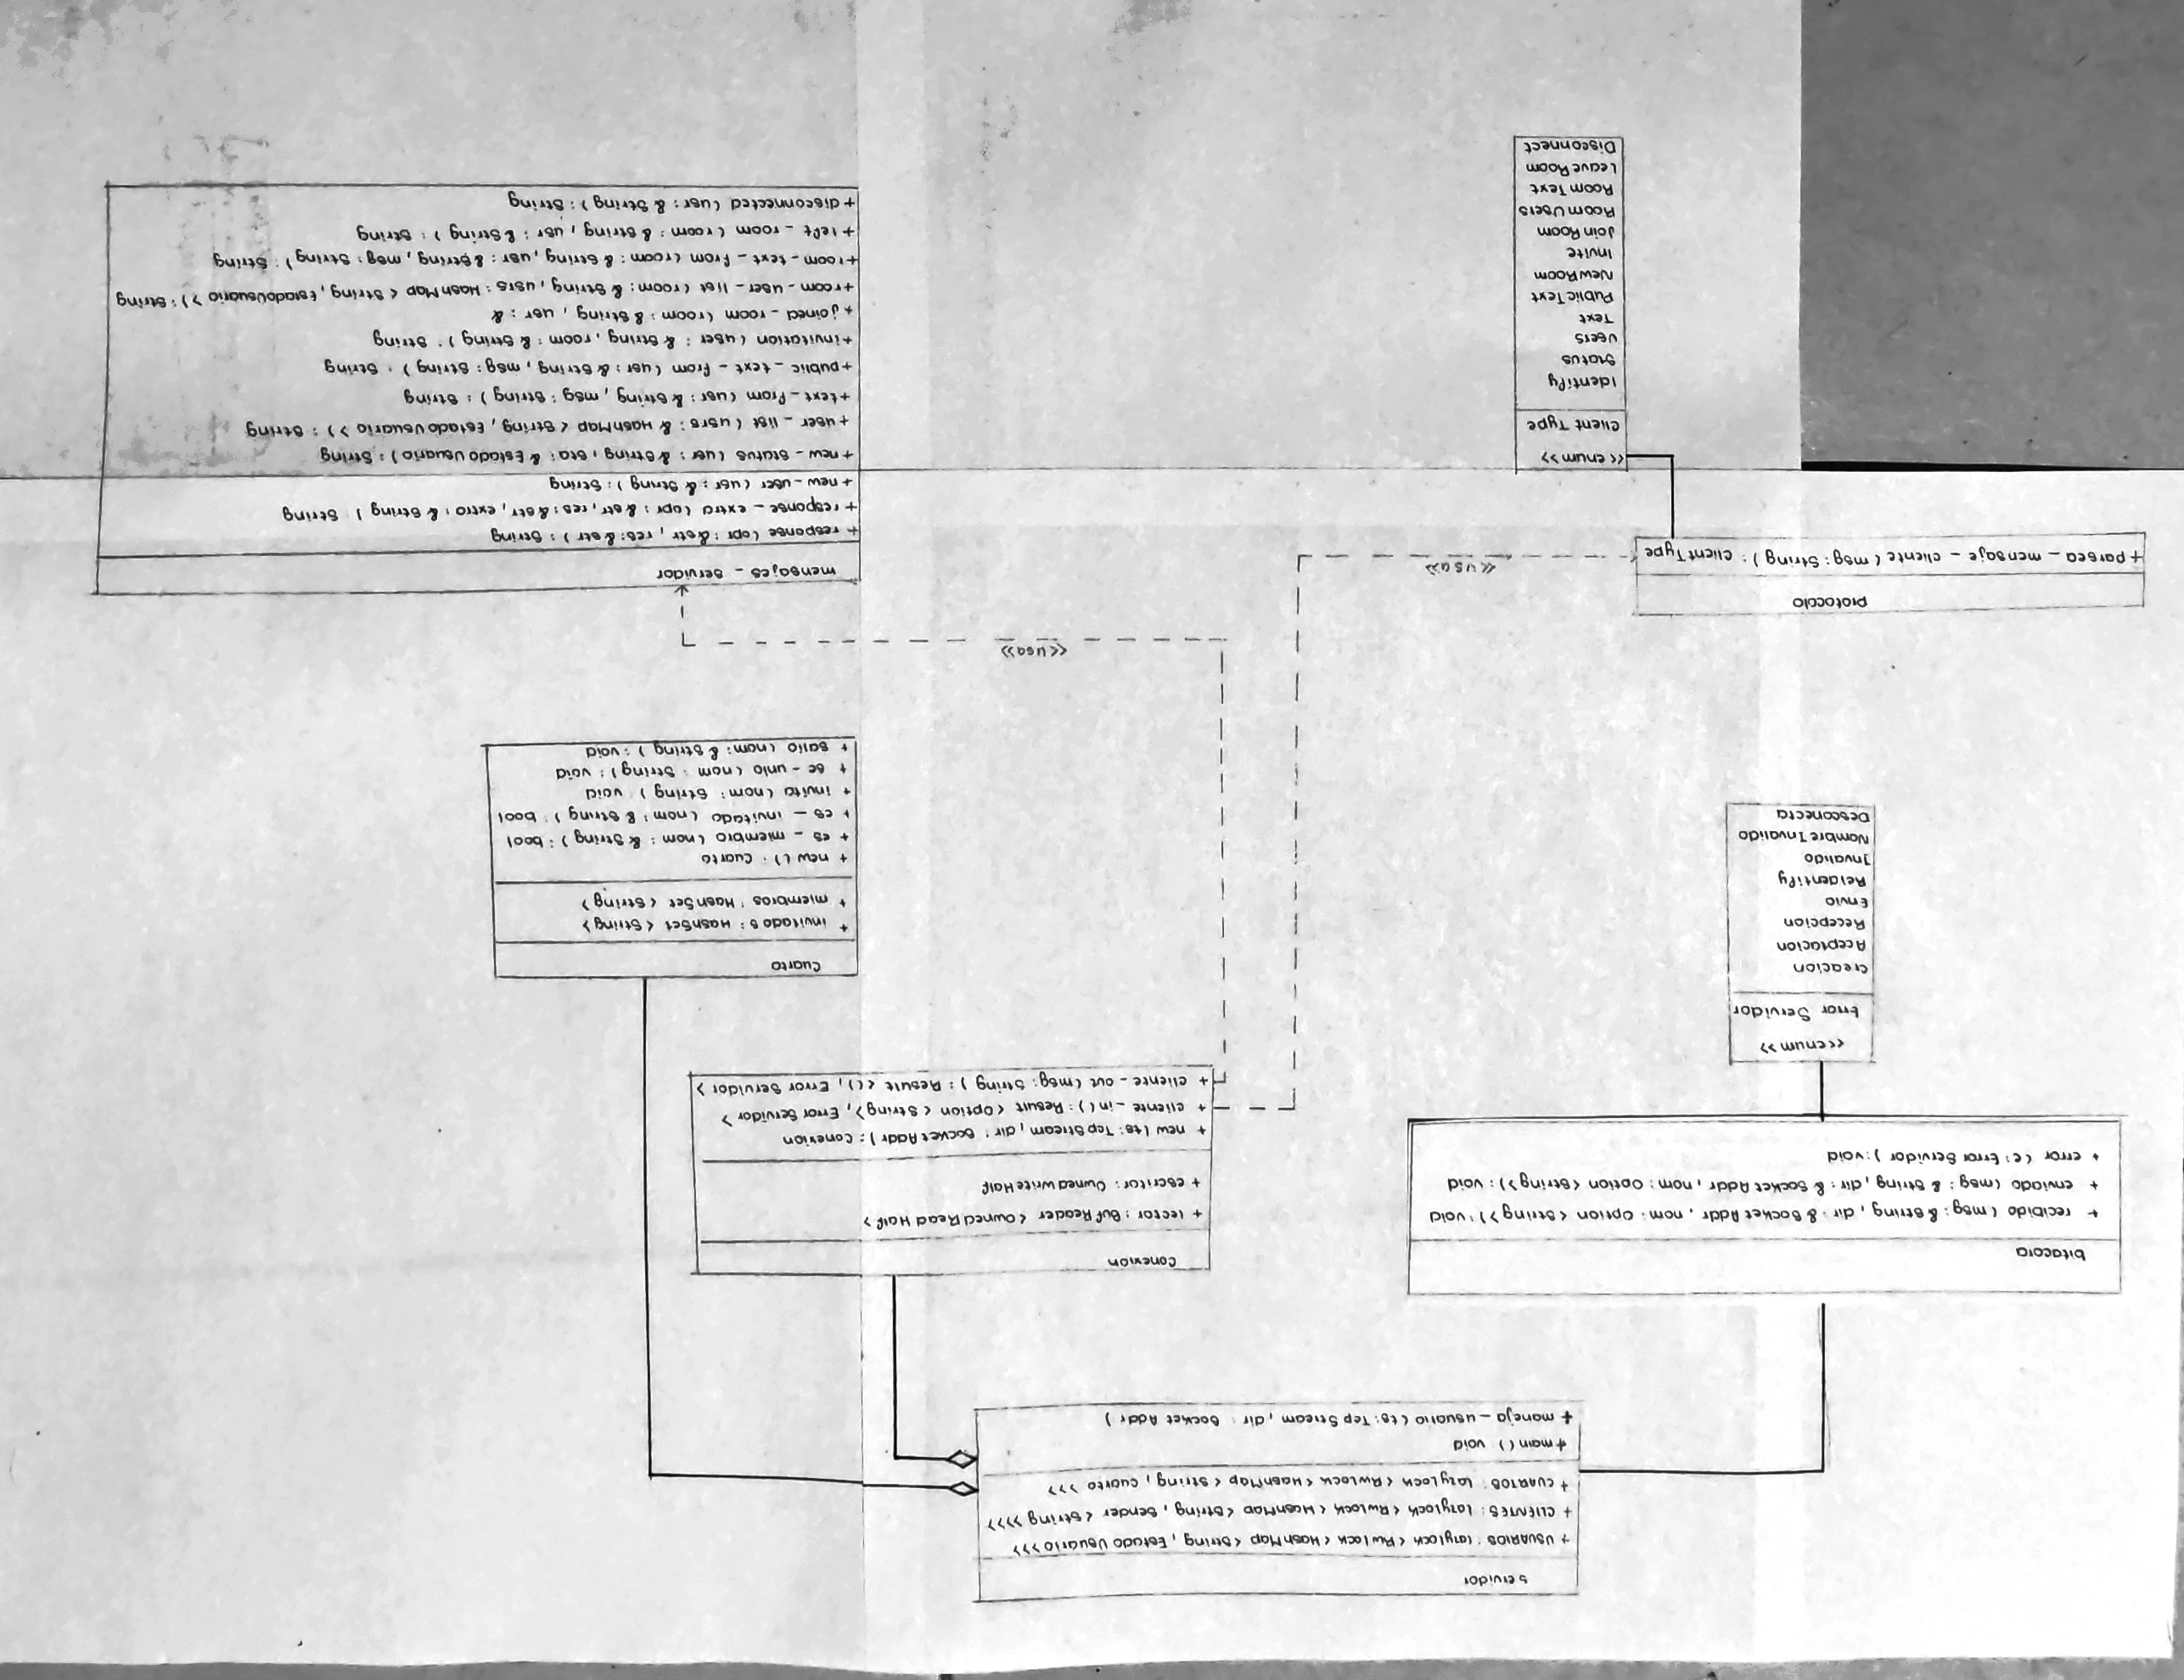
\includegraphics[width=0.7\textwidth, angle=180, origin=c]{servidor.jpg}
    \caption{Diagrama de clases del servidor.}
\end{figure}

\begin{figure}[H]
    \centering
    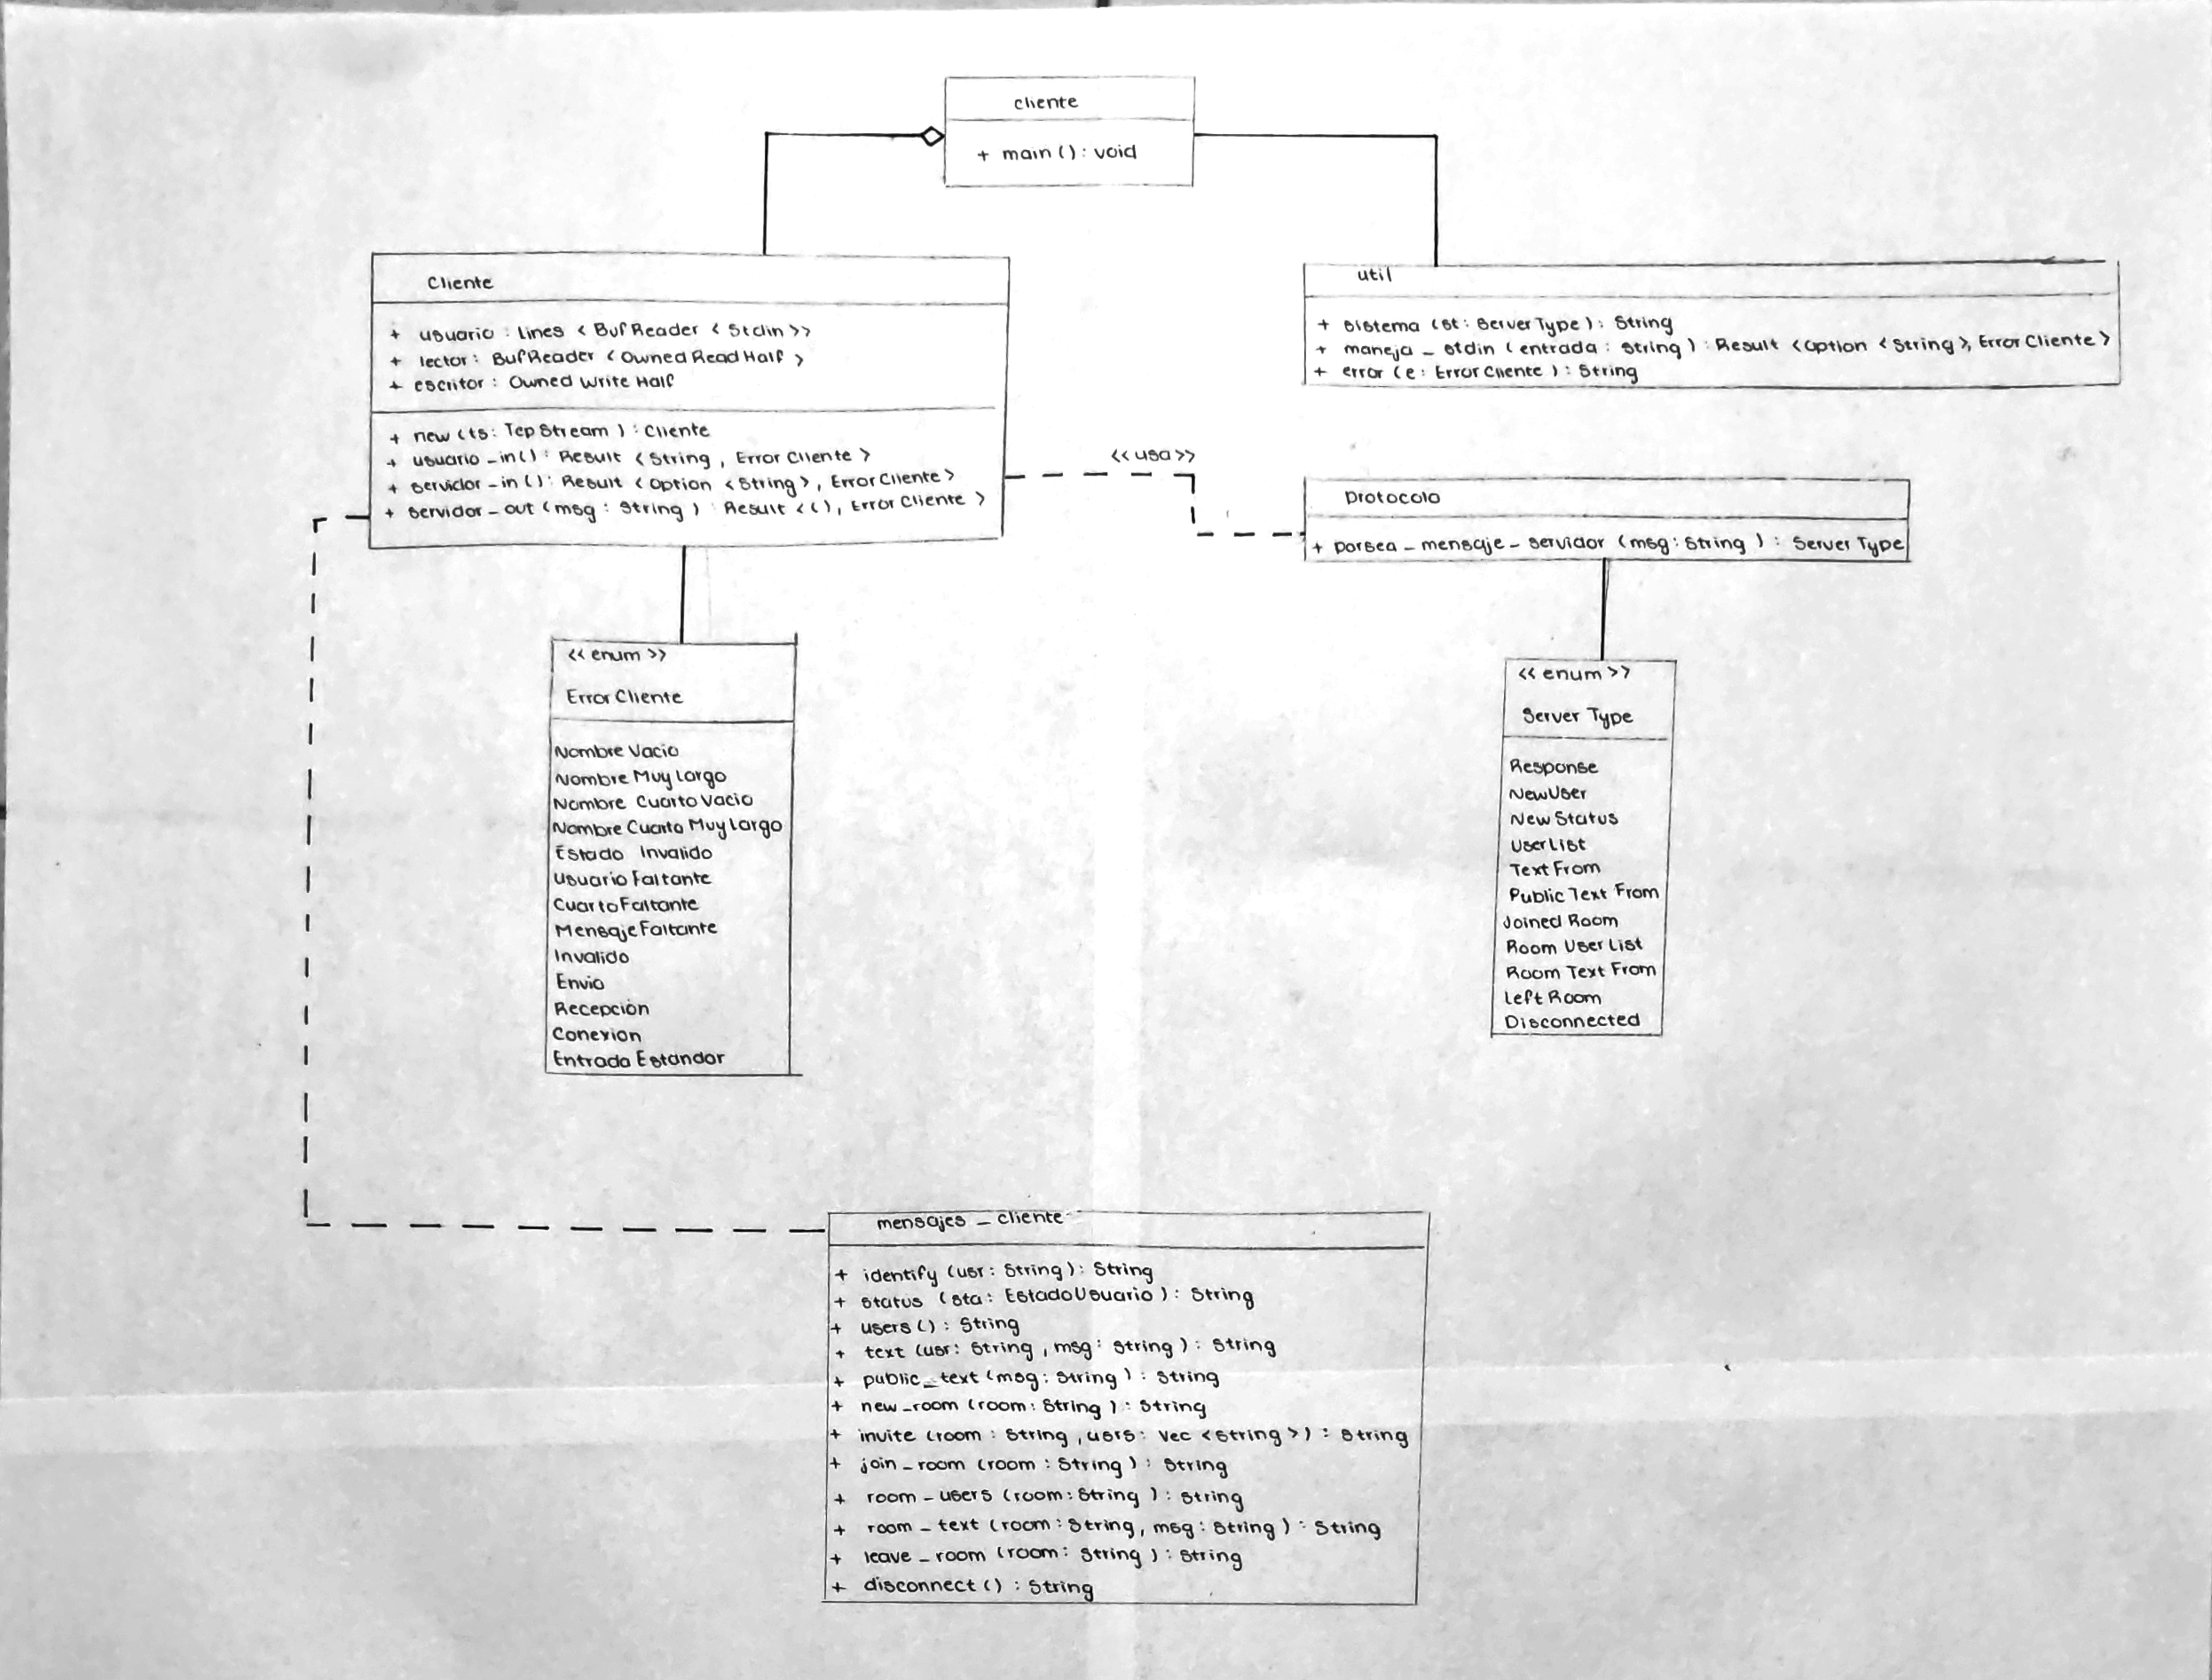
\includegraphics[width=0.7\textwidth]{cliente.jpg}
    \caption{Diagrama de clases del cliente.}
\end{figure}

\section{Conclusiones}
A pesar de que logré terminar con la implementación terminé no incluyendo una wiki y, como lo dejé para el último momento, no entendí cómo utilizar \textbf{Docker} y, por lo tanto, no lo incluí. Esas dos cosas serían lo único que vería necesario modificar sobre mi proyecto, sin embargo, desde otro punto de vista, me hubiera gustado cambiar las cosas en la siguiente lista:
\begin{itemize}
    \item Servidor
    \begin{itemize}
        \item Mover la estructura \textbf{Conexion} y sus métodos a la biblioteca compartida para poder hacer uso de ella en ambos binarios.
        \item Mover la función \textbf{maneja\_peticion} y sus funciones auxiliares al módulo \textbf{util} del servidor.
        \item Guardar los tres diccionarios dentro de una misma estructura y a su vez intentar juntar el diccionario de \textbf{Senders} con el de estados.
    \end{itemize}
    \item Cliente
    \begin{itemize}
        \item Separar la lógica de la entrada estándar en una estructura diferente, usar la estructura \textbf{Conexion} para la comunicación con el servidor.
        \item Mover la funciones \textbf{sistema} y sus funciones auxiliares a su propio módulo,
        \item Mover la enumeración \textbf{ErrorCliente} y la función \textbf{error} a su propio módulo.
        \item Mover la función para colorear una cadena a la biblioteca compartida.
        \item Cambiar el nombre del módulo \textbf{util} para reflejar que ahora solo tendría la función \textbf{maneja\_stdin} y sus funciones auxiliares.
    \end{itemize}
    \item Protocolo
    \begin{itemize}
        \item Mover \textbf{ClientType}, \textbf{ServerType} y sus respectivas funciones para parsear a sus respectivos módulos (\textbf{mensajes\_cliente} y \textbf{mensajes\_servidor}).
        \item Modificar el nombre de Protocolo a algo que denote que es simplemente una biblioteca compartida, de tal forma que el que se encuentre ahí la función para obtener la dirección IP tenga un poco más de sentido.
    \end{itemize}
\end{itemize}

\renewcommand{\refname}{Referencias}
\begin{thebibliography}{99}
\bibitem{rust-std}
The Rust Project Developers. (2026). \textit{The Rust programming language --- Standard library documentation}. \url{https://doc.rust-lang.org/std/}
\bibitem{rust-collections}
The Rust Project Developers. (2026). \textit{std::collections --- Rust standard library}. \url{https://doc.rust-lang.org/std/collections/index.html}
\bibitem{rust-hash}
The Rust Project Developers. (2026). \textit{std::hash --- Rust standard library}. \url{https://doc.rust-lang.org/std/hash/index.html}
\bibitem{rust-io}
The Rust Project Developers. (2026). \textit{std::io --- Rust standard library}. \url{https://doc.rust-lang.org/std/io/index.html}
\bibitem{rust-net}
The Rust Project Developers. (2026). \textit{std::net --- Rust standard library}. \url{https://doc.rust-lang.org/std/net/index.html}
\bibitem{rust-sync}
The Rust Project Developers. (2026). \textit{std::sync --- Rust standard library}. \url{https://doc.rust-lang.org/std/sync/index.html}
\bibitem{rust-env}
The Rust Project Developers. (2026). \textit{std::env --- Rust standard library}. \url{https://doc.rust-lang.org/std/env/index.html}
\bibitem{tokio}
Tokio Contributors. (2026). \textit{Tokio --- Asynchronous runtime for Rust}. \url{https://tokio.rs/}
\bibitem{tokio-io}
Tokio Contributors. (2026). \textit{tokio::io --- Tokio documentation}. \url{https://docs.rs/tokio/latest/tokio/io/index.html}
\bibitem{tokio-net}
Tokio Contributors. (2026). \textit{tokio::net --- Tokio documentation}. \url{https://docs.rs/tokio/latest/tokio/net/index.html}
\bibitem{tokio-sync}
Tokio Contributors. (2026). \textit{tokio::sync --- Tokio documentation}. \url{https://docs.rs/tokio/latest/tokio/sync/index.html}
\bibitem{serde}
Tolnay, D. (2025). \textit{serde --- Rust documentation}. \url{https://docs.rs/serde/latest/serde/}
\bibitem{serde-json}
Tolnay, D. (2026). \textit{serde\_json --- Rust documentation}. \url{https://docs.rs/serde_json/latest/serde_json/}
\bibitem{colored}
Thomas, T. (2026). \textit{colored --- Rust documentation}. \url{https://docs.rs/colored/latest/colored/}
\end{thebibliography}
\end{document}

